This chapter summarizes the efforts of writing Einstein Field equations
(EFE) \cite{Einstein15a,Einstein15b} in a way specially suitable for
high (convergence) order numerical integration, with the numerical
schemes presented in chapter~\ref{chapter:numerics}. For an introduction
into the problem and a review of previous work, see
Section~\vref{sec:gr-intro-intro}.
This chapter relies partially on the coauthored publications
 \cite{Dumbser2017} as well as \cite{Koeppel2017}.

\section{Motivation: The two body problem of GR}\label{sec:gr-intro}
Exact solutions of Einstein Field equations are ``rare'' \cite{Kramer80}
and well known solutions are highly symmetric spacetimes. Two astrophysically
relevant examples are the stationary Kerr black hole (two Killing vectors:
rotational / azimuthal and in time direction) and the static TOV solution of an
isotropic fluid in equilibrium (spherically symmetric, thus three orthogonal
spacelike Killing vectors)\footnote{
    The TOV solution is refered here synonmyously to as TOV star or neutron star.
    
	Particular spacetimes are introduced in the benchmark 
	sections,
	for instance the Kerr(-Schild) solution in 
	Section~\vref{sec:convergence-bh3d} and the TOV solution 
	in Section~\vref{sec:tov}. 
}.

\begin{marginfigure}
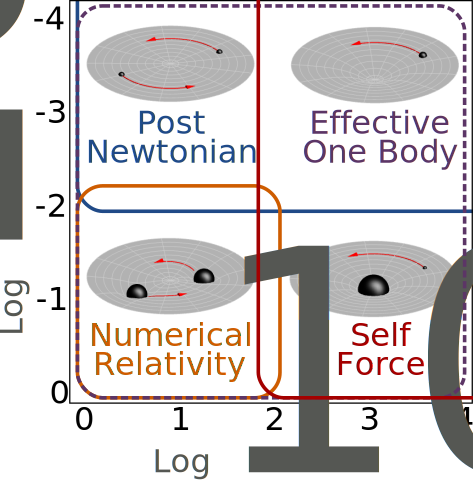
\includegraphics[width=\textwidth]{efe-intro-2body/2BodyEFE-SvenDrawing.pdf}
\caption[
  EFE 2body parameter space, drawn with Inkscape. \exclusive
]{
 Practicability/availability diagram of the two body problem in GR with
 the parameter range archieveable with approximations.
}
\label{fig:efe-intro-2body-paramspace}
\end{marginfigure}
%
Being a nonlinear theory where the superposition principle no longer holds (in contrast
to classical and quantum mechanics), the two body problem 
%for these two exemplaric objects
in (full) general relativity (GR) is nontrivial. That is, there is no way of analytically solving Einstein field
equations exactly for a spacetime holding two compact objects (black holes or neutron stars).
Instead, all attemps to find such spacetimes are using approximations which however
can be subsequently refined to converge to the real solution. The two major approximation
scales are
%\\
(1) the mass ratio $M_1/M_2$ of the two objects and
%\\
(2) the compactness $C=M/R$ of the system, with $R$ the object
seperation and $M=M_1+M_2$ the total spacetime mass
\cite{MTW1973,Wald84,Buonanno2014}. Due to the virial theorem, this
scale is similar to $v^2/c^2$ with the characteristic velocity $v$ of an object in the
binary system.

It is popular to inspect the two-dimensional space spanned by these two parameters
in a diagram (Figure \ref{fig:efe-intro-2body-paramspace}): Two perturbation theories
cover either the small compactness or the high mass ratio regime. The first one is
the Post Newtonian (PN) expansion of EFE where the velocity ratio is small compared to the speed
of light. The second one are gravitational self-force corrections \cite{Wald:2009ue} which
correct around an infinite mass ratio (static approximation of the heavier object /
test particle on a geodesic in an external metric).
Being analytic theories which approximate Einstein equations, for a given order of
approximation, these theories fail to describe a binary system with high mass, finite extend,
rapid rotation. In order to describe this strong gravity regime correctly, Einstein equations
must be solved without simplifying approximations. The answer from numerical relativity (NR) is to
approximate the spacetime itself instead of the field equations. The mathematical approach is
no more analytic but numerical, working on discretized fields, whereas the ``full'' Lagrangian
is solved, without the (computational/mathematical) need for a simplification.
\footnote{
It is interesting to do an excursion to the other popular nonlinear theory
in high energy physics, since there are similar approximations done: Quantum chromodynamics
(QCD), the special relativistic quantum theory of the strong force,
 part of the Standard Model of elementary particles and suitable for 
 describing, for instance,
 fundamental baryonic and mesonic particles hold together by the strong force.
The two body problem in QCD in the context of heavy quarks has a similiar parameter
space with similiar solutions: Instead of Post Newtonian
expansion, there is non-relativistic QCD, while the heavy quark effective theory is
renowed for describing dynamic quarks in the presence of infinetely heavy quarks. However,
in the relativistic regime of two quarks with similar mass, the full QCD Lagrangian must be
solved to predict correct observables. A successful theory to do so discretizes spacetime
(with periodic boundary conditions, therefore referred to as a ``lattice'') where
a QCD Lagrangian (not neccessarily describing all flavours) is solved
numerically. This research field is called Lattice QCD. At the present, numerical relativity and
lattice QCD are the two major challenging applications in high energy computational physics.
} % footnote
In practice, however, it is a long way to recast the Einstein field equations in a hyperbolic
way, suitable for ``time'' integration, and the following Sections will provide an
insight into the approach used within this work.

This broad-brush motivation for numerical approaches in field theory disregards
many successful attemps of covering the whole parameter space of Figure \ref{fig:efe-intro-2body-paramspace}
analytically. In case of GR, there is the effective one body formalism which is able of
an analytic treatment of the strong gravity regime of two body spacetimes by taking into
accounts results from PN and NR~\cite{Damour:2008yg,Buonanno:1998gg}. In contrast, numerical
relativity is the only approach to arbitrary strong gravity spacetimes which works from
first principles, \ie without any external input, and that can in principle cover the whole
space.

\section{The Cauchy Initial value formulation of GR}%
\label{sec:adm}%
%
General relativity is invariant under the Lorentz (Lie) group, that makes it a gauge
theory. The four degrees of freedom (DOF) from Lorentz group can be cast in 
general smooth coordinate transformations $x'_\mu = f_\mu(x)$ and this 
invariance is known as general or diffeomorphism covariance. From the
$4\times4=16$ components of Einstein equations, only 10 are independent, and
the gauge freedom removes another 4~DOF, thus 6 
physical DOF remain.

The ADM formulation (dating back to 1959 by Arnowitt, Deser, Misner
\cite{Arnowitt62}) is an Hamiltonian formulation of Einstein
field equations.
\footnote{
  We will refer to the ADM formulation synonymously to as the (Cauchy)
  initial value problem	formulation or the canonical formulation of EFE.
} It allows to define a time coordinate and thus to perform
a time evolution on the orthogonal spatial coordinates 
(\cf Section~\ref{sec:hamiltonian-motivation} on
Hamiltonian time evolution).
The ADM formulation is one way to identify/fix the gauge degrees of gravity
by dimensional reduction and restricting Einstein field equations on the
lower-dimensional hyperspaces (\eg $D=4$-dimensional spacetime is restricted on
3-dimensional hypersurfaces)\footnote{
	The ADM split, or rather the ADM canonical coordinates, are not a unique choice.
	The Ashtekar variables \cite{Ashtekar1986}, which rewrite three-dimensional slices into
	SU(2) gauge fields, are an example of a popular differen choice which is actually
	the foundation of loop quantum gravity \cite{Rovelli2008}.
}. Arbitrarily embedding $(D-1)$-mani\-folds within
a $D$-manifold can be described by a vector field $N_\mu$ with $D-1$ degrees of
freedom, thus this is a suitable method for gauge fixing.

The $D$-dimensional spacetime remains now as a gauge orbit. If the vector 
$N_\mu$ collects the gauge connections, one can arbitrarily select a direction
(for instance the first component of the vector $N_\mu$) and call it ``time''.
% wrong:
%\footnote{As a restriction, to properly interpret this direction as   
%	``timelike'', it should remain within the light cone to fulfill causality.}.

\subsection{Foliation of spacetime}\label{sec:adm-foliation}
The way to the classic 3+1 formulation of Einstein equations is typically
two-part: First, the geometry of foliations is specified by introducing a
number of tensors suitable for projecting four dimensional tensors onto
the submanifolds. Second, the projections are applied on Einsteins equations
and the resulting PDE system is discussed. This approach is proven and
part of modern numerical relativity books such as Alcubierre
\cite{Alcubierre:2008}, Bona and Palenzuela \cite{Bona2009},
Baumgarte and Shapiro \cite{Baumgarte2010}, Gourghoulhon
\cite{Gourgoulhon2012}, Rezzolla and Zanotti \cite{Rezzolla_book:2013}
or Shibata \cite{Shibata_book:2016}.

Given arbitrary gauge connections $N^\mu = (\alpha, \beta^\mu)$, time shall be
defined to advance along the vector $t^\mu = \alpha n^\mu + \beta^\mu$. This
motivates to define the normal vector to the spatial hypersurfaces $\Omega$
as $n^\mu = (1/\alpha, -\beta^i/\alpha)$ \footnote{
   Actually $t^\mu$ does \emph{not} need to be timelike, the only requirement
   is not to be tangential to to the spatial hypersurfaces
   \cite{Alcubierre:2008}.
   \\
   This is because the gauge choices are 
   arbitrary ($N_\mu \in \mathbb R$) and \ie a superluminal shift does not
   violate causality by principle.
}.

The line element shall commonly read $\d l^2 = \gamma_{ij} \d x^i \d x^j$,
the proper time along the normal vector (Eulerian observer) $\d \tau = \alpha 
\d t$. The induced three metric is identified as 
$\gamma_{\mu\nu} = g_{\mu\nu} + n_\mu n_\nu$ and the line element
thus $\d s^2= \alpha^2 \d t^2 + \gamma_{ij} (\d x^i + \beta^i \d t)(\d x^j + 
\beta^j \d t)$.

The extrinsic curvature describes how the submanifold is embedded in the outer
space and can be derived as $K_{\mu\nu} = -\nicefrac 12 \Lie_{\boldsymbol n} 
\gamma_{\mu\nu}$ wie Lie derivative along the normal direction $\boldsymbol n$,
which evaluates on purely spatial tensors as
\begin{equation}\label{eq:lie-normal}
\mathcal L_{\boldsymbol n} = \left( \mathcal L_{\boldsymbol t} - \mathcal L_\beta \right)
/ \alpha = \left(\partial_t - \beta^\mu \partial_\mu \right)/\alpha \,.
\end{equation}

It is worth mentioning that the original ADM group had a fairly different 
notation \cite{Gourgoulhon2012}, they derive the canonical conjugate momenta 
$\pi_{ij}$ instead of the extrinsic curvature $K_{ij} = 
-1/\sqrt{\gamma}(\pi_{ij} -
 \nicefrac 12 \gamma_{ij}\pi^m_m)$. The way 3+1 gravity is presented
in modern literature basically follows York \cite{York79}.

\begin{marginfigure}
	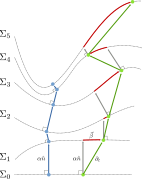
\includegraphics[width=\textwidth]{adm-definitions/adm-definitions.pdf}
	\caption[
	ADM definitions, drawn with Inkscape, \exclusive
	]{
		Cartoon for
		demonstrating the slicing (foliation) of 1+1 spacetime.
		The fixing of gauge freedoms is arbitrary and the shown example
		follows by intention no standard gauge fixing choice in NR.
		The foliation geometry is defined in continuum, this cartoon
		shows a number of different spatial hypersurfaces $\Sigma_i$,
		an exemplary normal vector fieldline (blue) 
		as well as an exemplary coordinate fieldline (green), determined
		by the time vector, which decomposes into spatial (shift) and
		temporal (lapse) direction. The lapse is the only spatial vector
		(``living on $\Sigma_i$''), while the other shown vectors are
		temporal. Since the vectors are shown non-bended, they shall be
		understood as infinitesimal.
	}
	\label{fig:efe-intro-2body-paramspace}
\end{marginfigure}%

\subsection*{3+1 split of the Energy momentum tensor}\label{sec.3p1-emtensor}
The normal vector $n_\mu$ as well as the spatial metric $\gamma_{ij}$ are
suitable for projecting four dimensional tensors into purely spatial or
purely temporal objects. Before this ``split'' is applied to Einstein equations
(Section~\ref{sec:3p1-split-efe}), it shall be applied to the Einstein source,
\ie the energy momentum tensor $T_{\mu\nu}$. Following the standard definitions,
the following four quantities, all measured by the Eulerian observer, shall be
defined:
\begin{align}
\label{eq:smunu.E}
E&=n^\alpha n^\beta T_{\alpha\beta}
\quad&&\text{the energy (momentum) density,}
\\
\label{eq:smunu.Si}
S_\alpha &= -\gamma^\mu_\alpha n^\nu T_{\mu\nu}
~~&&\text{the energy (momentum) flux,}
\\
\label{eq:smunu.Sij}
S_{\alpha\beta} &= \gamma^\mu_\alpha \gamma^\nu_\beta T_{\mu\nu}
\quad&&\text{the spatial energy momentum tensor and}
\\
S &= S^i_i 
\quad&&\text{its trace.}
\end{align}

\subsection[ADM equations]{3+1 split of Einstein Equations: ADM 
equations}\label{sec:3p1-split-efe}
The ADM split of Einsteins field equations is most readily obtained by
projection operators applied on EFE written as $G_{\mu\nu} - 8\pi T_{\mu\nu} = 0$
with the Einstein tensor 
$G_{\mu\nu} = R_{\mu\nu} + \nicefrac 12 R g_{\mu\nu}$ and the
Energy-Momentum-Tensor $T_{\mu\nu}$. Then, a full projection onto the normal
direction yields the Hamiltonian constraint equation
%\begin{subequations}\label{eq:adm-system}
\begin{equation}\label{eq:adm-system.hamiltonian}
0 = n_\mu n_\nu (G_{\mu\nu} - 8\pi T_{\mu\nu} ) = R - \tr(K^2) + (tr K)^2 - 16\pi~E
:= H
\end{equation}
Similarly, the three momentum constraints are derived by the
mixed projection:
\footnote{The notation $v_\alpha=(0,w_a)$ shall indicate that the 
  left hand side is four dimensional, while the right hand side is a purely
  spatial vector.}
\begin{equation}\label{eq:adm-system.momentum}
0 = \gamma_{\alpha\beta} n_\gamma (G_{\alpha\gamma} - 8\pi T_{\alpha\gamma} )
  = \left( 0, \nabla_k K^k_a - \nabla_a \tr K - 8\pi ~ S_a \right)
  := M_a
\end{equation}
$H=0$ and $M_a=0$
are the Hamiltonian and Momentum constraints, respectively, and their
deviation from zero (due to numerically introduced errors) is a measure to
assess the physicality of a system state.

The full projection onto the spatial hypersurface gives an evolution equation
for the extrinsic curvature,%
%\footnote{
%  Here it is convenient to project the Ricci tensor (following York
%  \cite{York79}) instead of the Einstein tensor (as ADM did).
%}
\begin{align}\label{eq:adm-system.kextr}
&  \gamma_{\alpha\beta} G^{\alpha\gamma} =
  \gamma_{\alpha\beta} 8\pi T^{\alpha\gamma} 
  \quad\Leftrightarrow\quad
  %(\partial_t - \Lie_{\bf \beta})
  \Lie_{\boldsymbol n} K_{ij} = \mathcal E_{ij}
  \,,
  \\
  \text{with}\quad
&   \mathcal E_{ij} = 
  - \nicefrac 1\alpha \nabla_i \nabla_j \alpha + 
  R_{ij} - 2 K_{ij} K^k_j + K K_{ij}
  - 8\pi \left( 
  S_{ij}  - \frac 12 \gamma_{ij} (S-E) \right)
  \nonumber
  \,.
\end{align}
The definition $K_{\mu\nu} = -\nicefrac 12 \mathcal L_{\boldsymbol n} 
\gamma_{\mu\nu}$ is already the evolution equation for $\gamma_{ij}$,
\begin{equation}\label{eq:adm-system.gamma}
\mathcal L_{\boldsymbol n} \gamma_{ij} = -2 K_{ij} \,.
\end{equation}
%\end{subequations}
The two evolution equations in $n^\mu$ direction can be transformed to
evolution equations using the ``time'' introduced in the previous section,
\ie \eqref{eq:lie-normal}.

The four equations (\ref{eq:adm-system.hamiltonian}-\ref{eq:adm-system.gamma})
are generally known as ADM equations.
With their 1+3 constraint equations and 6 evolution
equations\footnote{$\gamma_{ij}$ and $K_{ij}$ are symmetric 3-tensors with
	6~DOF each, however they are conjugate variables and therefore hold the 
	same information.}, they have the same 10~DOF as Einstein 
	field equations.

It is worthwhile to emphasize at this point that the constraint equations can
be used as Lagrangian Multipliers, for instance was $H$ already 
introduced
as Lagrangian multiplier in
$\Lie_{\boldsymbol n} K_{ij} = \mathcal E_{ij} - \gamma_{ij} H$ by 
York~\cite{York79}.
Obviously this does not change (continuum) physics, but the PDE
structure (system matrix) is a different one.

The ADM evolution equations are only weakly hyperbolic. This can be seen by
rewriting them as a first order formulation, fixing the gauges and showing
that parts of the system are not diagonizable \cite{Alcubierre:2008}.
As discussed in Section~\ref{sec:intro-eigensystems}, weakly hyperbolic PDEs
are not suitable for numerical integration since they are not well-posed.

\subsection{Gauge fixing}\label{sec:gauge-fixing}
\begin{marginfigure}[-2cm]
	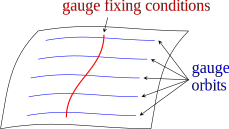
\includegraphics[width=\linewidth]{adm-gauge-orbits/gauge-orbits.pdf}
	\caption[Gauge orbits, \colorizedAfter{Meusburger:2010fs}
	]{
		Gauge fixing conditions must cut every gauge orbit 
		once. Every
		gauge orbit represents one physical solution which is 
		similar to
		another one. This generic sketch and language from 
		gauge theory can be
		mapped to GR/ADM language, a physical solution is a 
		particular
		coordinate system/slicing of spacetime.
		Colorized from~\cite{Meusburger:2010fs}.
	}
\end{marginfigure}%
In numerical relativity, gauge terms \emph{have} to be fixed since they appear
in the ADM system \eqref{eq:adm-system.kextr} and a numerical treatment requires
every variable to be represented by a number.

Physically, the effect of gauge fixing in the ADM split is equivalent to choose
a reference frame in GR (as it fixes the same four DOF). Fixing the lapse $\alpha$ determines the foliation and time coordinates
(``slicing conditions'') while fixing the shift $\beta^i$ chooses the spatial
coordinates. The gauge freedom can be
used to move coordinates in a desirable way throught the simulation domain which itself
can make the three-dimensional evolution equations more hyperbolic or more
elliptic \cite{Gourgoulhon2012}, but they can even be (dynamically) evolved
by a PDE and thus extend the overall evolution system\footnote{
 That means their PDEs neccessarily have to be taken into account when
 making an eigenanalysis of the particular 3+1 formulation of Einsteins
 equation (refering to modification of ADM equations, as presented
 in the subsequent sections).
}.

\subsection*{Slicing conditions}
Slicing conditions can be time-locally defined by constraining ADM quantities,
for instance the maximal slicing condition where $K^i_i = 0$. This maximises
the volume of the spatial hypersurface (hence the name) and has singularity
avoiding features, \ie $\alpha\to0$ when $t \to \infty$. It yields an
elliptic equation for the lapse $\alpha$ which makes it unsuitable for
time evolutions\footnote{This is because the elliptic equation 
	(which has no time derivatives) has to be solved at every timestep.
	There are however approximations by parabolic laws
	\cite{Shibata99a,Shibata_book:2016}.
}. Being maximal sliced is a property of a single hypersurface. In constrast,
slicing conditions which are defined via the lapse (or coordinates)
characterize a series of hypersurfaces and are not meaningful for single
hypersurfaces~\cite{Gourgoulhon2012}, because in general the lapse has no
meaning on a single hypersurface\footnote{However, given a prescribed
	gauge-fixing law, the lapse can \emph{be given} meaning even on a single
	hypersurface.
}

There is also the class of algebraic slicing conditions which directly determine
the lapse function and do not require to solve a (differential) equation
(at least not for constructing the initial data/initial slice). The most
simple example of this class is geodesic slicing, where $\alpha:=1$.
It got its name from the worldlines of Eulerian observers, which can be shown
to be geodesic. Their eigentime $\tau=t$ is equivalent to coordinate time.

Harmonic slicing is the most likely a gauge which is comparable to
Lorentz gauge ($\partial_\mu A^\mu=0$ with gauge field $A^\mu$ in 
electrodynamics and related field theories). It can be defined as imposing
the gauge $\nabla_\mu \nabla^\mu x^\alpha = 0$ on the coordinates. This
translates the Laplace equation $\nabla_\mu \nabla^\mu t=0$ in 3+1 formalism,
\ie the time coordinate has a harmonic solution. It is a special
case of $1+\log$/Bona Masso slicing, which is given by 
\cite{Bona95b}
\begin{equation}\label{eq:bona-masso}
(\partial_t - \Lie_\beta) \alpha = -(K-K_0) \alpha^2 f(\alpha)
\end{equation}
where $f(\alpha)=0$ gives geodesic slicing, $f(\alpha)=1$ gives harmonic
slicing and $f(\alpha)=2/\alpha$ gives ``1+log''-slicing, which gets it
name from the special case $\beta=0$ where \eqref{eq:bona-masso} reduces
to $\partial_t \alpha=\partial_t \ln |\gamma|$ which has the solution
$\alpha=1+\ln |\gamma|$. 1+log slicing has even better singulatiry avoidance
properties then harmonic slicing but can penetrate horizons (in Schwarzschild
spacetime), furthermore it mimics maximal slicing. Here, a
formulation with $K_0=K(t_0)$ the extrinsic curvature trace at beginning of the
simulation is given, which can help to preserve maximally sliced initial
data. Most worth mentioning, \eqref{eq:bona-masso} is a hyperbolic
conservation law for the lapse, which makes it an interesting addition to
a 3+1 evolution system.

\subsection*{Spatial gauges}
Fixing the temporal gauge freedom $\alpha$ determines the arrow of time at any
spatial hypersurface, since time is defined differentially between spatial
hypersurfaces. Instead, fixing the three gauge freedoms $\beta^i$ determines only
the propagations of coordinates between the hypersurfaces but leaves the choice of
coordinates for instance at the initial data hypersurface undetermined. This is because
the gauge connections $(\alpha, \beta^i)$ are only meaningful
quantities \emph{inbetween} two spatial hypersurfaces\footnote{
	In fact, there exist also \emph{full} spatial coordinate-fixing choices but they
	are not discussed here.
}.

Similar to the geodesic slicing, there is the Eulerian gauge $\beta^i=0$ as then
$x^i=$const are the worldlines of an Eulerian observer. As soon as the spacetime
is non-static, better more tailored spatial coordinates might be wanted. One
example are minimal distortion gauges which try to minimize the change of the
(conformal) 3-metric.
They yield in an elliptic equation for the shift. However,
minimal distortion gauges are interesting for the wave zone in a merger event,
basically because they are adapted to the way how gravitational waves are defined
and extracted (Appendix~\ref{sec:extracting-gws}).

Most interesting for this monograph are the Gamma freezing and Gamma driver
shift conditions. The first one is a simplification of approximative (pseudo)
minimal distortion gauges and can be formulated as\footnote{
	Here, the tilde in $\tilde{\gamma}$ and $\tilde{\Gamma}$ indicate 
	\emph{conformal} quantities as introduced in Section~\vref{sec:bssn}.
	Especially, the contracted Christoffel symbol is an evolution quantity
	in the BSSNOK system.
}
\begin{equation}
\partial_t \tilde{\Gamma}^i = 0, \quad\text{with}~~
\tilde{\Gamma}^i := \tilde{\gamma}^{jk} \left(\tilde{\Gamma^i}_{jk} - \tilde{\Gamma^i}_{jk} \right)
\end{equation}
An elliptic equation for the shift can be derived which must be fulfilled. By
further modifying the minimal distortion law, a parabolic \cite{Alcubierre00a}
and eventually a hyperbolic \cite{Alcubierre02a,Lindblom:2003ad,Bona05a}
alternative has been found, which reads in first order 
formulation
\begin{equation}\label{eq:gamma-driver}
	\partial_t \beta^i = \frac 34 b^i + \beta^k \partial_k \beta^i
	\quad\text{and}\quad
	\partial_t b^i = \partial_t \tilde\Gamma^i - \eta b^i + \beta^k \partial_k 
	b^i
\end{equation}
with a positive function $k$, a dissipation/damping coefficient $\eta$ and $b^i$ the
auxilliary field required for the first order rewrite
\cite{Baker:2006mp,Brugmann:2008zz}. Typical values are $k=3/4$ and
$\eta=1$ or $\eta\sim M/M_0$ with $M$ the ADM mass measured in multiples of the
unit mass $M_0$ (\ie $M_0=\Msol$ in astrophysical spacetimes).

The gamma driver shift condition turned out to be very successful for moving puncture
solutions and is, as part of the BSSNOK equations as presented in the next section,
an ``industry standard'' for stable general relativistic evolutions of compact object
mergers.

\section{The BSSNOK equations}\label{sec:bssn}

The Baumgarte-Shapiro-Shibata-Nakamura-Oohara-Kojima
(BSSNOK) formulation \cite{Shibata95,Baumgarte99,Nakamura87,Brown09},
is a hyperbolic formulation of Einsteins Equations in the
3+1 split. Hyperbolicitiy is archived with several ``tricks'' added to the
ADM system. These are primarily a conformal transformation of the ADM
state variabels $\gamma_{ij}, K_{ij} \to \tilde{\gamma}_{ij}, \tilde A_{ij}$,
the addition of the constraint equations $H=M_i=0$ to the evolution equations,
the addition of slicing conditions and Gamma driver to the evolved equations
and the seperate evolution of several quantities such as the extrinsic curvature
trace $K$, a contracted Christoffel symbol and the conformal factor. The
evolved variables of the BSSNOK system are therefore
\begin{equation}\label{eq:bssnok-evol-quantities}
\begin{aligned}
&\gammat_{ij} := e^{-4\phi} \gamma_{ij}
\,,\quad\quad
\Atilde_{ij} := e^{-4\phi} \TraceFree{K_{ij}} :=
e^{-4\phi}
\left( K_{ij} - \frac 13 \gamma_{ij} K \right)
\,,
\\
&\Phi := \frac{1}{12} \ln(\gamma) 
\,,\quad
K  := \gamma^{ij} K_{ij}
\quad\text{and}\quad
\Gtilde^i := \gammat^{jk} \Gtilde^i_{jk}
\,,
\end{aligned}
\end{equation}
where $\gammat_{ij}$ is the conformal 3-metric,
\begin{equation}
\tilde{\Gamma}^i_{jk} := \frac{1}{2} \gammat^{ab} \left(
\partial_{j} \gammat_{kb} + \partial_k \gammat_{jb} - \partial_b \gammat_{jk}
\right)
\end{equation}
are the Christoffel symbols associated with this metric and $\tilde{\Gamma}^i$
the freely evolved contraction of this symbol. $\Phi$ is the conformal factor
(see Section~\ref{sec:conformal-factor}) split off
the metric. $\tilde A_{ij}$ is the conformal trace-free extrinsic curature tensor which
is evolved in place of $K_{ij}$. Furthermore, with suitable slicing conditions
and the Gamma driver, lapse $\alpha$, shift $\beta^i$ and an auxillary field $b^i$
is evolved.

\subsection{Covariance of the BSSNOK formulation}
All new evolution fields $\Psi, K, \tilde{\Gamma}^i$ are pure gauge quantities
\cite{Baumgarte99}. The scalars $\Psi$ and $K$ are derived from tensors,
however $\tilde{\Gamma}^i$ does not transform like a vector, since the connection
coefficients $\Gamma^i_{jk}$ do not. Therefore, the BSSNOK equations are not
(fully) covariant.
However, the difference between two Christoffel symbols in a coordinate change
transforms like a tensor field \cite{Gourgoulhon2012}. % P.243
That is, if one introduces a background metric $\mathring{\gamma}_{ij}$
and a new metric $\epsilon_{ij} = \tilde{\gamma}_{ij} - \mathring{\gamma}_{ij}$, then
the Christoffel symbols of the new metric,
$\Delta^i_{kl} = \tilde{\Gamma}^i_{kl} - \mathring{\gamma}^i_{kl}$
and the derived $\hat{\mathring\Gamma}^i$ does so, too.
For BSSNOK, a system like this was introduced in \cite{Ruchlin2017} in 
order to evolve Einstein field equations on spherical and singular coordinate systems.
\footnote{Appendix \ref{sec:fo-fccz4} deepens this issue for the presented
  FO-CCZ4 formulation in this chapter.}

\subsection{Definitions for the conformal factor}%
\label{sec:conformal-factor}
% section comes from my document 
%Antelope/doc/conformal-treatment.pdf

A key concept in BSSNOK is splitting off a conformal factor, recognizing
that the three-metric $\gamma_{ij}$ and three-extrinsic curvature $K_{ij}$
are part of a conformal equivalence class. Evolving a fundamental representation
does not only have an advantage in conformally flat spacetimes but in fact
it was shown by York \cite{York71,York72} that a traceless and tranverse
tensor carries the true degrees of freedom of the gravitational field
\cite{Gourgoulhon2012}. Therefore, the concept was picked up by various
other formulations of Einsteins equations and especially by various
technical implementations, sometimes with subtle differences in the definition,
usually due to technical reasons (like positivity preserving techniques) which 
promise better numerical stability. In order to clarify the definitions, some
intermediate symbols shall be defined. First of all, any (rank 2)
tensor, for instance the 3-metric $\gamma_{ij}$, has a corresponding tensor 
density $\gammat_{ij}=\gamma^{n/2}\gamma_{ij}$ with weight $n\in\mathbb R$
and determinant $\gamma=\det(\gamma_{ij})$~\cite{Gourgoulhon2012}. The weight of
the three metric is $n=2/3$ and therefore, the conformal factor $\Omega$ can be
introduced as
\begin{equation}
\Omega = \gamma^{1/3}
\quad\text{so that}\quad \gamma_{ij} = \Omega ~ \gammat_{ij}
\end{equation}
In literature, the notation $\psi^4 \equiv \Omega$ is more widespread
\footnote{to be explicit, in $\psi^4$, the~$\cdot^4$ is an exponent, not an 
index. This symbol should not be mixed up with the Weyl scalar $\psi_4$,
where the $\cdot_4$ is really an index.% The Weyl scalar is popular in
%numerical relativity for extracting gravitational waves
%(Appendix~\vref{sec:extracting-gws}).
}, thus
$\gamma = \psi^{12}$. The following three popular but different choices are
widespread in literature
\footnote{This choice is motivated due to the implementation of all three
 variants in the \code{Antelope} code (see Section \vref{sec:fo-ccz4-implementations}).
}, formalized by a function $f(\Omega)$, or $f(\psi^4)$,
respectively. It is then $\gamma_{ij} = f^{-1} ~ \gammat_{ij}$. The three
choices $f\in\{ \xi, \Phi, W \}$ are\footnote{
  Within the BSSNOK community, the choice $f=\Phi$ is popular (and was
  made here in the text), while for instance \cite{Shibata_book:2016}
  uses $f=W$ and \cite{Hilditch2012} uses $f=\xi$.
}
%
%\begin{subequations}
\begin{alignat}{8} % was 10
\xi (\Omega) &= \Omega^{-1}  &&= \psi^{-4} &&= \gamma^{-1/3} \,,
&&\quad\text{then}~~ \gamma_{ij} = \xi^{-1}~ \gammat_{ij}
%&&\quad \texttt{(ifdef XI)} 
\label{eq:conformal-factor-Xi}
\\
\Phi  (\Omega) &= \log \Omega^3 &&= \log \psi &&= \frac 1{12} \log \gamma \,,
&&\quad\text{then}~~ \gamma_{ij} = e^{4\Phi}~ \gammat_{ij}
%&&\quad \texttt{(ifdef PHI)}
\label{eq:conformal-factor-Phi}
\\
W     (\Omega) &= \Omega^{-1/2} &&= \psi^{-2} &&= \gamma^{-1/6} \,,
&&\quad\text{then}~~ \gamma_{ij} = W^{-2}~ \gammat_{ij}
%&&\quad \texttt{(default)}
\label{eq:conformal-factor-W}
\end{alignat}
%\end{subequations}
%
However, the choice of a particular $f$ does not necessarily mean that this 
quantity
is evolved. In fact, the notation used for the FO-CCZ4 system
(Section~\ref{sec:fo-ccz4}) uses choice \eqref{eq:conformal-factor-W}
but calls $W(\Omega) =: \phi$. However, $\phi$ is treated as a
\emph{primitive} variable which is converted to a \emph{conserved}
variable where $\log \phi = \log W = - \nicefrac 16 \log \gamma$, which however
does not meet any standard definitions of
(\ref{eq:conformal-factor-Xi}-\ref{eq:conformal-factor-W})

\subsection[Evolution equations]{The BSSNOK evolution equations}
The BSSNOK equations are given by (see \cite{Brown09} for a derivation)
\begin{fullwidth} % tufte
%	\begin{subequations}
		\begin{align}
		\label{eq:bssn-phi}
		\left(\partial_t - \Lie_{\beta} \right) \Phi
		&=
		\frac 16 \partial_k \beta^k - \frac 16 \alpha K
		\\
        \label{eq:bssn-gammat}
		\left(\partial_t - \Lie_{\beta} \right) \gammat_{ij}
		&=
		-2\alpha \Atilde_{ij} - \frac 23 \gammat_{ij} \partial_k \beta^k
		\\
        \label{eq:bssn-K}
		\left(\partial_t - \Lie_{\beta} \right) K
		&=
		\alpha \left( \Atilde_{ij} \Atilde^{ij} + \frac 13 K^2 \right)
		- \gamma^{ij} \nabla_i \nabla_j \alpha
		+ 4\pi (S^k_k + E)
		\\
        \label{eq:bssn-Atilde}
		\left(\partial_t - \Lie_{\beta} \right) \Atilde_{ij}
		&=
		e^{-4\Phi} \TraceFree{\alpha(R_{ij} - 8\pi S_{ij}) - \nabla_i \nabla_j 
		\alpha}
		- \frac 23 \Atilde_{ij} \partial_k \beta^k + \alpha \left(K 
		\Atilde_{ij} - 2\Atilde_{ik} \Atilde^k_j \right)
		\\
        \label{eq:bssn-Gtilde}
		\left(\partial_t - \Lie_{\beta} \right) \Gtilde^i
		&=
		\gammat^{kl} \partial_k \partial_l \beta^i
		+ \frac 23 \gammat^{jk} \Gtilde^i_{jk} \partial_l \beta^l
		+ \frac 13 \nabla^i \partial_k \beta^k
		- 2 \Atilde^{ik} \partial_k \alpha
		%\\
		%&\phantom{=}
		+ 2 \alpha \Atilde^{kl} \Gtilde^i_{kl}
		+ 12 \alpha \Atilde^{ik} \partial_k \phi
		- \frac 43 \alpha \tilde\nabla^i K
		- 16\pi \alpha \gammat^{ij} S_j
		\raisetag{32pt}
		\\
        \label{eq:bssn-alpha}
		\left(\partial_t - \Lie_{\beta} \right) \alpha
		&=
		-2 \alpha K
		\\
        \label{eq:bssn-beta}
	    (\partial_t - \Lie_{\beta}) \beta^i
		&=
		\frac 34 b^i
		\\
        \label{eq:bssn-auxB}
	    (\partial_t - \Lie_{\beta}) b^i
		&=
		\partial_t \Gtilde^i - \eta b^i
		\end{align}
%	\end{subequations}
\end{fullwidth}
with the covariant derivative $\tilde{\nabla}$ with respect to $\gammat_{ij}$
\footnote{Here, only terms $\tilde{\nabla}_i A=\partial_i A$
	and $\tilde{\nabla}_i B_j = \partial_i B_j - \tilde{\Gamma}^k_{ij} B_k$ appear.
},
Lie derivative $\Lie_{\beta} = \beta^k \partial_k$\footnote{
	Conventionally, the ADM system is typically displayed as
	$\Lie_{\boldsymbol{n}} X = \mathcal R(X)$ while the BSSNOK and 
	subsequent systems are typically displayed as
	$(\partial_t - \Lie_{\beta}) X = \alpha \mathcal R(X)$.
}, the trace-free operator $\TraceFree{T_{ij}}$ defined as in 
\eqref{eq:bssnok-evol-quantities}, and $(E,S_i,S_{ij})$ being 
the spatial parts of the energy momentum tensor as defined in
(\ref{eq:smunu.E}-\ref{eq:smunu.Sij}). In this equation system, there
are especially two very lengthy abbreviations used: First, the
3-Ricci tensor in \eqref{eq:bssn-Atilde} which is defined with the conformal
decomposition $R_{ij} := \tilde R_{ij}^\Phi + \tilde R_{ij}$ as%
\footnote{Elaborate splits of ``helper'' quantities (\ie tensors derived from
evolution quantities) will become even more present in the FO-CCZ4 system.}
\begin{align}\label{eq.bssnok.conformalR}
\tilde R_{ij}^\Phi 
&=
\Phi^{-2} \left[
\Phi \left( \tilde\nabla_i \tilde\nabla_j \Phi
+ \gammat_{ij} \tilde\nabla^k \tilde\nabla_j \Phi \right)
- 2 \gammat_{ij} \tilde\nabla^k \tilde\nabla_k \Phi \right] \,,
\\
\tilde R_{ij}
&=
- \frac 12 \gammat^{lm} \partial_l \partial_m \gammat_{ij}
+ \gammat_{k(i} \partial_{j)} \Gtilde^k
+ \Gtilde^k \Gtilde_{(ij)k} + \gammat^{lm}
\left[ 2 \Gtilde^k_{l(i} \Gtilde_{j)km} 
+ \Gtilde^k_{im} \Gtilde_{kjl} \right] \,,
\nonumber
\end{align}
and second, the time-derivative of $\tilde{\Gamma}^i$ in \eqref{eq:bssn-auxB}
which refers to \eqref{eq:bssn-Gtilde}.

The evolution system also contains PDEs for the lapse $\alpha$ and shift
vector $\beta^i$, in this particular case the famous Bona-Masso type slicing
conditions.

For the numerical intergration, a partly constrainted approach is used at every
time step to impose that \footnote{In practice, this means a modification of 
 the state vector before or after every timestep.}
\begin{equation}
\det(\gammat_{ij}) = 1 \quad\text{and}\quad \operatorname{tr}(\Atilde_{ij}) = 0
\end{equation}
Similiar to ADM equations, the BSSNOK system is first order in time and second
in space, for a proof of hyperbolicity it must be brought into first order in
time and space (this was done in \cite{Beyer:2004sv} for a large number of
slicing conditions). Notably, for a fixed (non-evolved) shift vector
$\beta^i$, BSSNOK is symmetric hyperbolic. Since its first publication,
BSSNOK was quite successful for its robustness in numerical simulations and
got an ``industry standard'' for numerical relativistic time evolutions of
astrophysical spacetimes.

%Note the added Hamiltonian and momentum constraints on the RHS in order to
%guarantee hyperbolicity of the system.

%In the same publication, a different definition of hyperbolicity
%also proofs the second order version of BSSNOK strongly hyperbolic for any
%shift condition.

\section{The Z4 family and CCZ4}\label{sec:Z4-family}
The Z4 formulation of Einstein field equations (EFE) was formulated by Bona,
Ledvinka, Palenzuela, Zacek \cite{Bona:2003fj,Bona:2003qn}. They recognize that
in ADM formalism, the discrimination of the constraint equations
(\ref{eq:adm-system.hamiltonian},\ref{eq:adm-system.momentum}) versus the 
evolution equations
(\ref{eq:adm-system.kextr},\ref{eq:adm-system.gamma})
in a ``naive'' unconstrained evolution breaks general covariance. In Z4,
the derivative of a zero vector $Z_\mu=0$ \footnote{$Z_\mu=0$ motivates the 
name: A ``zero'' vector of length 4,	hence ``Z4''. The vector vanishes 
analytically but gets non-zero in numerical simulations.} is added to the field 
equations as a generalized Lagrangian multiplier (GLM)
which then read in trace-reversed form \cite{Bona:2003fj}
\begin{equation}\label{eq:z4-efe}
R_{\mu\nu} + 2\nabla_{(\mu} Z_{\nu)} = 8\pi \left( T_{\mu\nu} - \frac 12 T 
g_{\mu\nu} \right) \,.
\end{equation}
The field equations can also be derived from a minimal action principle
\cite{Bona:2010is}. They are first order in time, second order in space for the
metric, first order in space for $Z_\mu$. 
\footnote{The actual evolution equations are given later compact for all
	proposed members of the Z4 family.}
In the 3+1 split, with $Z_\mu = (\theta / \alpha, Z_i)$, the two new
evolution quantities for $\theta$ and $Z_i$ cannot be discriminated against
the ones for $\gamma_{ij}$ and $K_{ij}$ and thus general covariance is
maintained. Notably, these two new evolution equations take the place of the
ADM constraint equations, because $Z_\mu=0$ are four constraints and
non-zero values of $Z_\mu$ measure the ``physicality'' of an approximated
(numerical) solution. This is  a \emph{different} measure for
error than the regular
ADM Hamiltonian and momentum constraint (violations)
(\ref{eq:adm-system.hamiltonian},\ref{eq:adm-system.momentum}) which of course
still can be determined similarly also in the Z4 system, independently
of the $Z_\mu$ vector \footnote{For a comparison of the quality of 
 different formulations of EFEs, it is
 useful to fall back to $(H,M_i)$ as the ``lowest common denominator'',
 which always can be computed.}. The resulting PDE system is then almost similar
to the ADM equations (\ref{eq:adm-system.hamiltonian}-\ref{eq:adm-system.gamma}), namely
\begin{fullwidth}% tufte
\begin{align}
	\left(\partial_t - \Lie_{\beta} \right) \gammat_{ij}
	&=
	-2\alpha K_{ij}
	\\
	\left(\partial_t - \Lie_{\beta} \right) K_{ij}
	&=
	-\nabla_i \nabla_j \alpha
	+ \alpha \left[ R_{ij} - 2 K_{ij} K^k_j + (K-2\Theta)K_{ij}
	%- \NewTerms{\kappa_1(1+\kappa_2)\Theta\gamma_{ij}}
	\right]
	%\\
	%&\phantom{=}
	- 8\pi\alpha \left[ S_{ij} - \frac 12 \gamma_{ij} (S-E) \right] 
	\\
	\left(\partial_t - \Lie_{\beta} \right) \Theta
	&=
	\frac \alpha 2 \left[
	R + 2 \nabla_k Z^k + (K - 2\Theta)K - K_{ij} K^{ij}
	\right]
	- Z_k \nabla_k \alpha  
	% -\NewTerms{2\kappa_1(2+\kappa_2)\Theta} 
	- 16 \pi E
	\\
	\left(\partial_t - \Lie_{\beta} \right) Z_i
	&=
	\alpha \left[ \nabla_j (K_i^j - \delta_i^j K)
	+ \partial_i \Theta - 2 K_i^j Z_j \right]
	- \Theta \nabla_i \alpha
	% - \NewTerms{\kappa_1 Z_i}
	- 8\pi S_i
	\end{align}
\end{fullwidth}
%
The first order version of Z4 was brought into a conservative form and is
proven to be strongly hyperbolic~\cite{Alic:2009}.
The main drawbacks of the Z4 formulation is the lack of the 
Gamma driver
\eqref{eq:gamma-driver}, \ie there are no good gauges which 
result in horizon 
growth in black hole simulations.

% Recovery of BSSNOK and KST is possible \cite{Kidder01a}
%
\subsection[Z4c]{Conformal Z4 (Z4c)}
The conformal Z4 (Z4c) version was developed as a conformal but non-covariant
extension to Z4 \cite{Bernuzzi:2009ex,Cao:2012,Ruiz:2010qj,Weyhausen:2011cg,Hilditch2012}.
The modified EFEs
\begin{equation}\label{eq:Z4c}
R_{\mu\nu} + 2\nabla_{(\mu} Z_{\mu)}
=
8\pi (T_{\mu\nu} - \frac 12 T g_{\mu\nu})
+ \kappa_1 \left[ 2 n_{(\mu} Z_{\nu)} - (1 + \kappa_2) g_{\mu\nu} n_\sigma Z^\sigma \right]
\end{equation}
differ from the Z4 equations \eqref{eq:z4-efe} only by the algebraic damping
terms on the RHS, modulated by $\kappa_1$ and $\kappa_2$ which determine the damping
amplitude used to drive the growth of constraint violations to zero.
In the 3+1 split the Z4c formulation discard a number of terms which renders the
evolution equations non-covariant but very close to BSSNOK.
\todo[color=green]{
    Z4c: It would be nice to better work out the differences between Z4c and CCZ4.
    Especially since we have Z4c implemented in Antelope, also the practical difference
    is of interest, such as cost, Exactness. This would all be part of the frequently
    discussed code comparison paper which is however out of scope in the moment.
}
The resulting system is provably strongly hyperbolic for usual gauge choices.

The addition of the damping terms allows to advect and (if desired) damp
nonzero constraints which appeared during evolution. The consequence is of
course that the numerical solution stays much closer to a physical one, which is
especially helpful for very long running simulations (compared to the average
wave speed, \ie the speed of light, or the  mass of the spacetime, respectively).
The typical text-book motivation for this
mechanism employs Gauss law in electromagnetism, \ie preserving the solenoidal magnetic
field $\vec \nabla \cdot \vec B=0$, where the GLM is introduced as \cite{Dedner:2002}
\begin{alignat}{3}
\partial_t B^i &= \mathcal  R
&&\quad\Rightarrow\quad  \partial_t B^i = \mathcal R - \partial^i \psi \\
\partial_i B^i &= 0
&&\quad\Rightarrow\quad  \partial_i B^i = \mathcal  D(\psi) = 
c_\text{cleaning}^{-2} \partial_t \psi
\end{alignat}
In this minimal example, there is an evolution equation for the vector $B^i$ 
with a
spatial differential operator $\mathcal R = \mathcal R(B^i, \partial_i B^j, 
\dots)$.
The new evolved scalar $\psi$ couples the divergence freedom ($\partial_i 
B^i=0$)
to the evolution equation, following a differential operator $\mathcal D$. A 
hyperbolic
choice for this operator results in an advection quation for $\psi$.
~In a similar way, in Z4c, the four fields $(\Theta,Z_i)$ play the role of $\psi$
in this example.\footnote{
  See section \ref{sec:divergence-cleaning} for divergence cleaning
  techniques in magnetohydrodynamics.
}

%$\partial_i A^i = 0$ becomes instead $\partial_t A^i = \phi$ and
%$\partial_t \phi = \partial_t A^i$

\subsection[SO-CCZ4]{Conformal and covariant Z4: (SO-)CCZ4}
The CCZ4 (conformal and covariant Z4) system was developed to address
the non-covariant property of Z4c~\cite{Alic:2011a}. The derivation starts with 
the same field equations \eqref{eq:Z4c} but do not discard terms at the 3+1 split.
\footnote{
  Thus, the property ``covariant'' in CCZ4/Z4c is to be understood as
  ``beeing \emph{more} covariant then Z4''. However, as CCZ4 takes over the
  non-covariant ``conformal connection functions'' $\tilde{\Gamma}^i$ from
  BSSNOK (Section \ref{sec:bssn}), CCZ4 is not covariant.
  Appendix \ref{sec:fo-fccz4} briefly presents a \emph{fully} covariant CCZ4
  system which implements the ideas of \cite{Ruchlin2017}.
}

The conformal transformation applied in CCZ4 is similar to the BSSNOK one but
usually given with a different conformal factor (here $f=W$ from 
Section~\ref{sec:conformal-factor}),
\begin{equation}
\begin{aligned}
W      &:=  \gamma^{-\nicefrac 16}  \,,
&
K      &:=  \gamma^{ij} K_{ij}  \,,
\\
\gammat_{ij}  &:= W^2 \gamma_{ij}  \,,\quad
&
\Atilde_{ij}  &:= W^2 \TraceFree{K}  \,,
\\
\Gtilde^i     &:= \gammat^{jk} \Gtilde^i_{jk}  \,,
&
\Ghat^i       &:= \Gtilde^i + 2 \gammat^{ij} Z_j   \,,
\end{aligned}
\end{equation}
In CCZ4, the new symbol $\hat{\Gamma}^i$ replaces $Z_i$ as evolution quantity, while
$\Theta=Z_0$ remains an evolution quantity.

%
The full CCZ4 system in 3+1 split is given by
\cite{Alic2013,Alic:2011a}
\begin{fullwidth}
\begin{eqnarray}
%
\partial_t\tilde\gamma_{ij} &=& - 2\alpha \tilde A_{ij}
+ 2\tilde\gamma_{k(i}\partial_{j)}~\beta^k
- \frac{2}{3}\tilde\gamma_{ij}\partial_k~\beta^k
+\beta^k \partial_k \tilde\gamma_{ij} \,,  \label{gamma_eq}\\
%
\partial_t \tilde A_{ij} &=& \phi^2  \left[-\nabla_i \nabla_j 
\alpha
+ \alpha \left(R_{ij} + \nabla_i Z_j + \nabla_j Z_i - 8 \pi S_{ij}
\right)\right]^{\rm TF}
+ \alpha \tilde A_{ij}\left(K- 2\Theta\right) \nonumber \\
&&
- 2\alpha \tilde A_{il}\tilde A^l_j %\nonumber  \\
+ 2\tilde A_{k(i}\partial_{j)}~\beta^k
-\frac{2}{3}\tilde A_{ij}\partial_k~\beta^k + \beta^k 
\partial_k \tilde A_{ij}  \,,  \label{A_eq} \\
%
\partial_t\phi &=& \frac{1}{3} \alpha \phi K
- \frac{1}{3} \phi \partial_k \beta^k + \beta^k \partial_k \phi 
\,, \label{phi_eq} \\
%
\partial_t K &=& - \nabla^i \nabla_i \alpha + \alpha \left(R + 2
\nabla_i Z^i + K^2 -2 \Theta K \right)
+ \beta^j \partial_j K - 3 \alpha \kappa_1 \left(1 +
\kappa_2\right) \Theta  + 4 \pi \alpha \left(S - 3 \tau\right)
\,, \\
%
\partial_t \Theta &=& \frac{\alpha}{2}  \left[R + 2 \nabla_i 
Z^i - \tilde A_{ij} \tilde
A^{ij} + \frac{2}{3} K^2 - 2 \Theta K\right] - Z^i
\partial_i \alpha+ \beta^k \partial_k \Theta
- \alpha \kappa_1 \left(2 + \kappa_2\right) \Theta  - 8\pi 
\alpha\,\tau
\,,
\phantom{aaa}% avoid the tag to be ontop of tau
\\
%
\partial_t \hat\Gamma^i &=& 2\alpha \left[\tilde\Gamma^i_{jk} 
\tilde A^{jk}
- 3 \tilde A^{ij} \frac{\partial_j \phi}{\phi} - \frac{2}{3}
\tilde\gamma^{ij} \partial_j K \right]
+2\tilde\gamma^{ki}\left(\alpha \partial_k \Theta - \Theta
\partial_k \alpha
- \frac{2}{3} \alpha K Z_k\right) -  2\tilde A^{ij} \partial_j 
\alpha
\nonumber \\
&& + \tilde\gamma^{kl} \partial_k \partial_l \beta^i
+ \frac{1}{3}\tilde\gamma^{ik}\partial_k\partial_l \beta^l
+ \frac{2}{3} \tilde\Gamma^i \partial_k \beta^k -
\tilde\Gamma^k \partial_k \beta^i
+ 2 \kappa_3 \left(\frac{2}{3} \tilde\gamma^{ij} Z_j \partial_k 
\beta^k -
\tilde\gamma^{jk} Z_j \partial_k \beta^i \right)
\nonumber \\
&&  + \beta^k \partial_k \hat\Gamma^i 
- 16 \pi \alpha  \tilde\gamma^{ij} S_{j}
- 2 \alpha \kappa_1 \tilde \gamma^{ij} Z_j
\,, \label{Gamma_eq}
\\
%
\label{1plog}
\partial_t \alpha &=& - \alpha^2 g(\alpha) \left(K - K_0 - 
2\Theta \right) + \beta^k \partial_k \alpha \,, \\
%
\label{gammadriver1}
\partial_t \beta^i &=& f b^i +\beta^k\partial_k\beta^i \,, \\
%
\label{gammadriver2}
\partial_t b^i &=& \partial_t \hat\Gamma^i - \beta^k \partial_k 
\hat\Gamma^i
+ \beta^k\partial_k b^i - \eta b^i \,,
\end{eqnarray}
\end{fullwidth}
Here, again, the Gamma driver and Bona-Masso slicing conditions were added,
as in the case for the BSSNOK equations.
